\documentclass[man]{apa6}\usepackage[]{graphicx}\usepackage[]{color}
%% maxwidth is the original width if it is less than linewidth
%% otherwise use linewidth (to make sure the graphics do not exceed the margin)
\makeatletter
\def\maxwidth{ %
  \ifdim\Gin@nat@width>\linewidth
    \linewidth
  \else
    \Gin@nat@width
  \fi
}
\makeatother

\definecolor{fgcolor}{rgb}{0.345, 0.345, 0.345}
\newcommand{\hlnum}[1]{\textcolor[rgb]{0.686,0.059,0.569}{#1}}%
\newcommand{\hlstr}[1]{\textcolor[rgb]{0.192,0.494,0.8}{#1}}%
\newcommand{\hlcom}[1]{\textcolor[rgb]{0.678,0.584,0.686}{\textit{#1}}}%
\newcommand{\hlopt}[1]{\textcolor[rgb]{0,0,0}{#1}}%
\newcommand{\hlstd}[1]{\textcolor[rgb]{0.345,0.345,0.345}{#1}}%
\newcommand{\hlkwa}[1]{\textcolor[rgb]{0.161,0.373,0.58}{\textbf{#1}}}%
\newcommand{\hlkwb}[1]{\textcolor[rgb]{0.69,0.353,0.396}{#1}}%
\newcommand{\hlkwc}[1]{\textcolor[rgb]{0.333,0.667,0.333}{#1}}%
\newcommand{\hlkwd}[1]{\textcolor[rgb]{0.737,0.353,0.396}{\textbf{#1}}}%

\usepackage{framed}
\makeatletter
\newenvironment{kframe}{%
 \def\at@end@of@kframe{}%
 \ifinner\ifhmode%
  \def\at@end@of@kframe{\end{minipage}}%
  \begin{minipage}{\columnwidth}%
 \fi\fi%
 \def\FrameCommand##1{\hskip\@totalleftmargin \hskip-\fboxsep
 \colorbox{shadecolor}{##1}\hskip-\fboxsep
     % There is no \\@totalrightmargin, so:
     \hskip-\linewidth \hskip-\@totalleftmargin \hskip\columnwidth}%
 \MakeFramed {\advance\hsize-\width
   \@totalleftmargin\z@ \linewidth\hsize
   \@setminipage}}%
 {\par\unskip\endMakeFramed%
 \at@end@of@kframe}
\makeatother

\definecolor{shadecolor}{rgb}{.97, .97, .97}
\definecolor{messagecolor}{rgb}{0, 0, 0}
\definecolor{warningcolor}{rgb}{1, 0, 1}
\definecolor{errorcolor}{rgb}{1, 0, 0}
\newenvironment{knitrout}{}{} % an empty environment to be redefined in TeX

\usepackage{alltt}

\title{Always Use the Separate Variances t Test for Two Independent Groups}
\shorttitle{Separate Variances t Test}
\author{Joshua D. Wondra and Richard Gonzalez}
\affiliation{University of Michigan}

\abstract{This is an abstract}
\keywords{t test, new statistics}
\IfFileExists{upquote.sty}{\usepackage{upquote}}{}
\begin{document}
\maketitle

This is an introduction

\section{Method}


\section{Results}



We report the observed Type I error rates, observed power, and coverage probability for the classic and separate variance t tests.

\subsection{Type I Error Rates}
In this section we report type I error rates for the classic and separate variance t tests when the null hypothesis is true. Prior research has demonstrated that when either sample sizes or variances are equal, the type I error rates are preserved at .05 for both tests (CITATIONS). 

\subsubsection{Equal Variances, Different Sample Sizes}
Consistent with prior research, the type I error rate was .05 for both the classic and separate variance t tests across all sample sizes and sample size ratios.

\subsubsection{Equal Sample Sizes, Different Variances}
Consistent with prior research, the type I error rate was .05 for both the classic and separate variance t tests across all sample sizes and variance ratios.

\subsubsection{Different Sample Sizes, Different Variances}
Consistent with prior research, the classic t test was not robust when both variances and sample sizes were equal. When the group with the bigger sample also had the bigger variance, the classic t test was more conservative; the type I error rate dropped as low as .01 when the large group had twice the sample size and five times the variance of the small group (see Figure 1). 

\begin{knitrout}
\definecolor{shadecolor}{rgb}{0.969, 0.969, 0.969}\color{fgcolor}
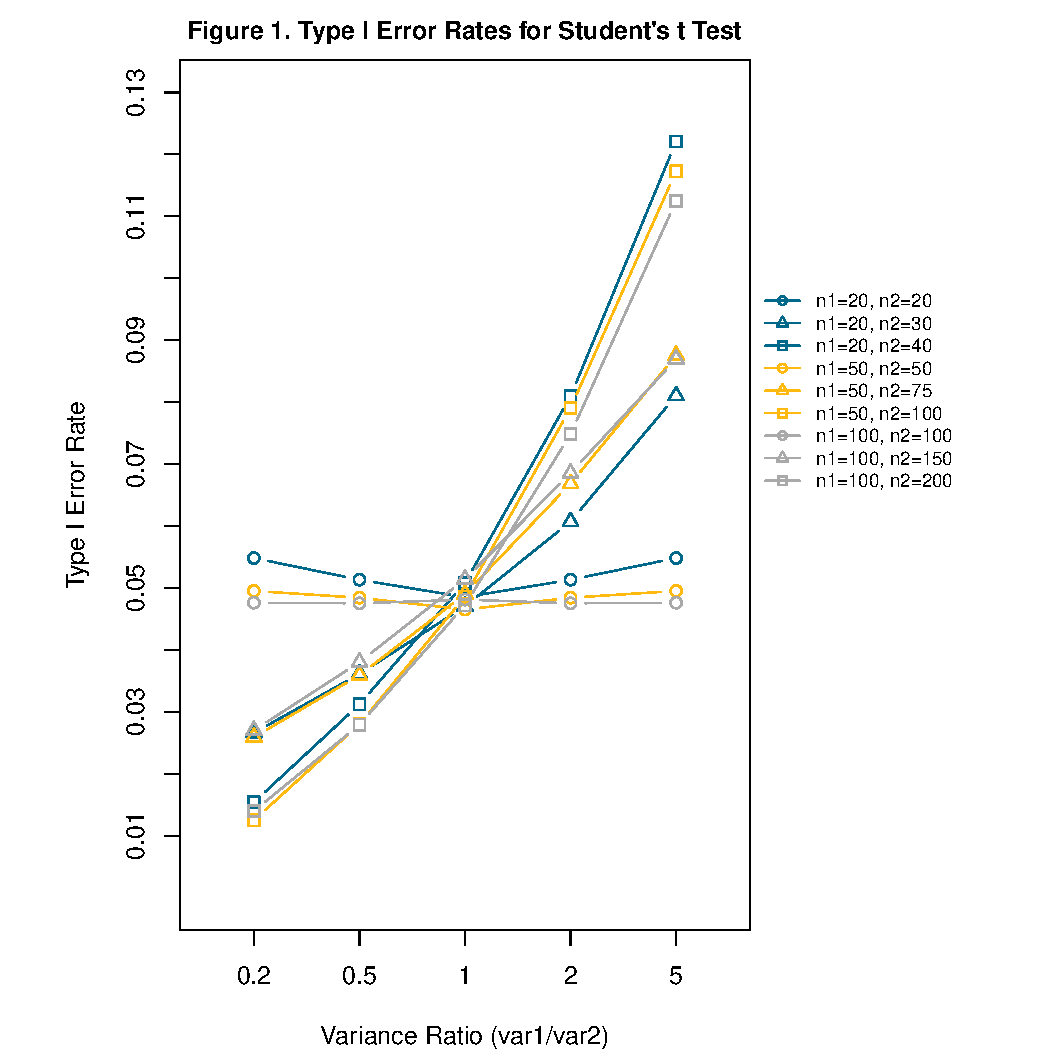
\includegraphics[width=\maxwidth]{figure/ssv_type11} 

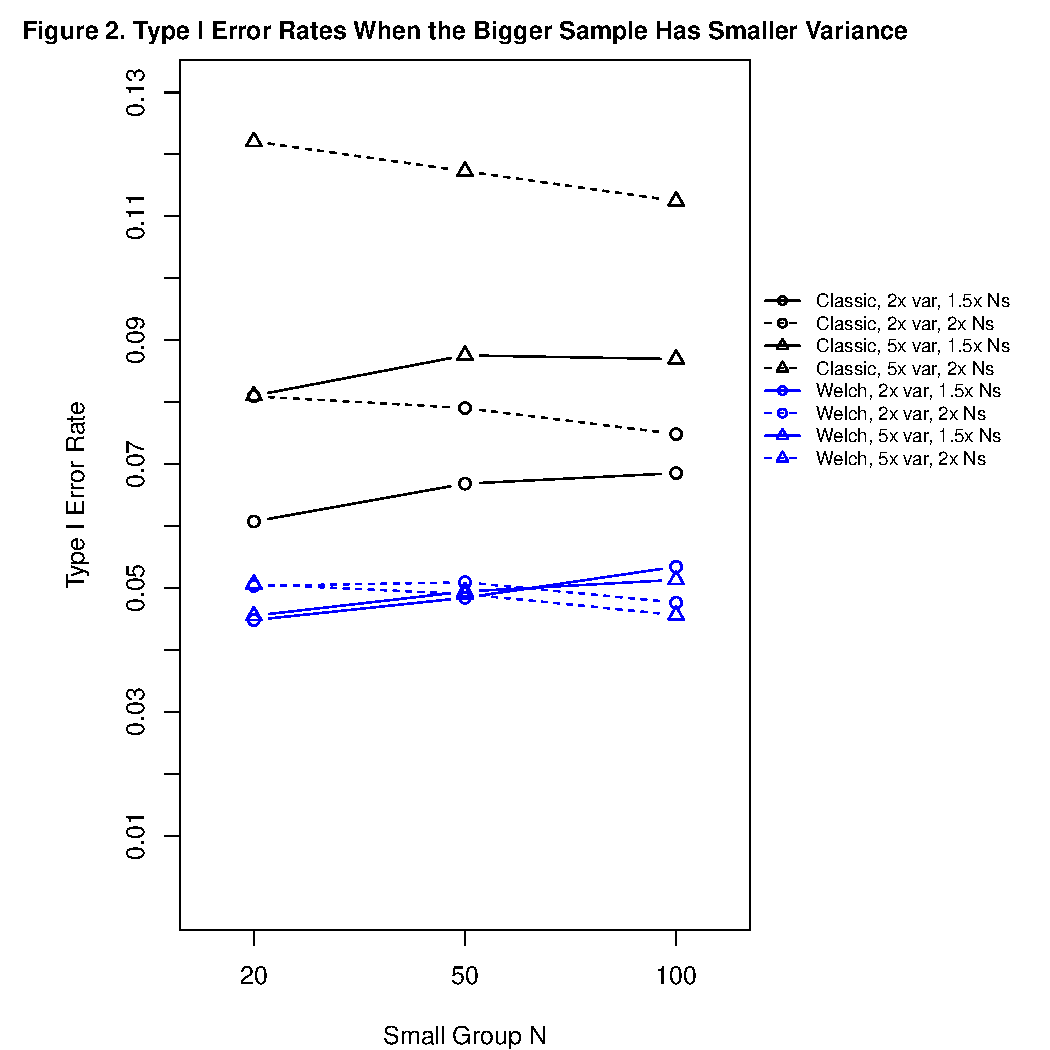
\includegraphics[width=\maxwidth]{figure/ssv_type12} 

\end{knitrout}
When the group with the bigger sample had the smaller variance, however, the classic t test was more liberal; the type I error rate inflated to just over .12 when the large group had twice the sample size and five times the variance of the small group (see Figure 2). In all cases, however, the separate variances t test approximately  maintained the expected type I error rate of .05.

\begin{knitrout}
\definecolor{shadecolor}{rgb}{0.969, 0.969, 0.969}\color{fgcolor}
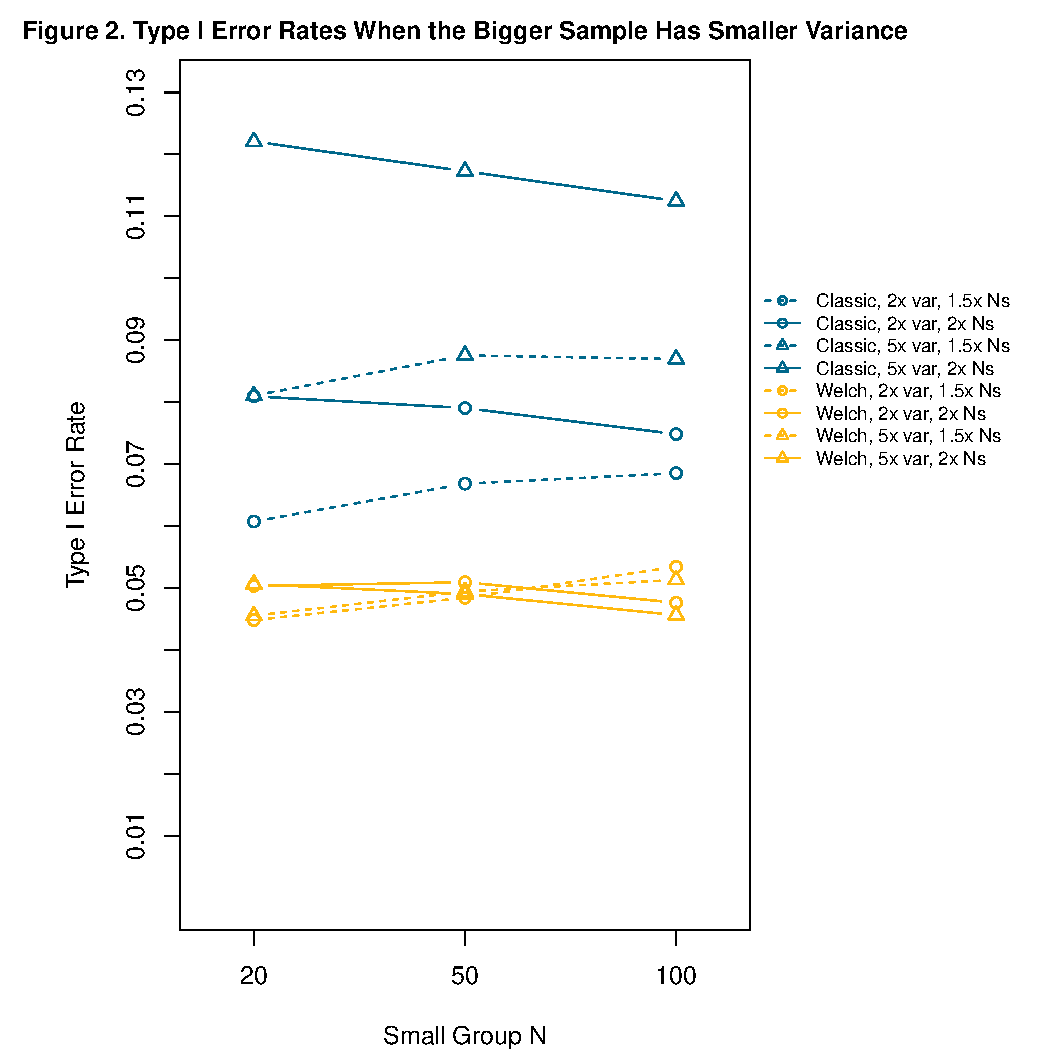
\includegraphics[width=\maxwidth]{figure/bsv_type1} 

\end{knitrout}
In summary, the type I error rates for the classic t test were quite variable when both sample sizes and variances were unequal between the two groups. In contrast, the type I error rates for the separate variances t test were mostly consistent with the expected .05 rate.

\subsection{Power}
In this section we report observed power rates for the classic and separate variance t tests when the null hypothesis is true. Prior research has focused on Type I error rates, but it has not examined whether choosing the separate variance t test also results in a loss of power to detect true effects. We examined power differences in the two tests when the sample sizes and variances are unequal. We looked at the power of the tests to detect small, medium, and large effects based on Cohen's d and compared it to the expected power based on an assumption of equal variances. This means that for the baseline comparison when variances were unequal, we treated it as though the difference in variance is due to sampling error rather than a true population difference. As with Type I errors, there were no differences between the classic and separate variance tests when sample sizes and variances were equal.

\subsubsection{Equal Variances, Different Sample Sizes}
Figure 3 displays the observed power for the classic and separate variance tests when sample sizes and sample size ratios varied, but variances were equal. As with Type I errors, the differences in the proportion of rejected null hypotheses was negligible. 

\begin{knitrout}
\definecolor{shadecolor}{rgb}{0.969, 0.969, 0.969}\color{fgcolor}
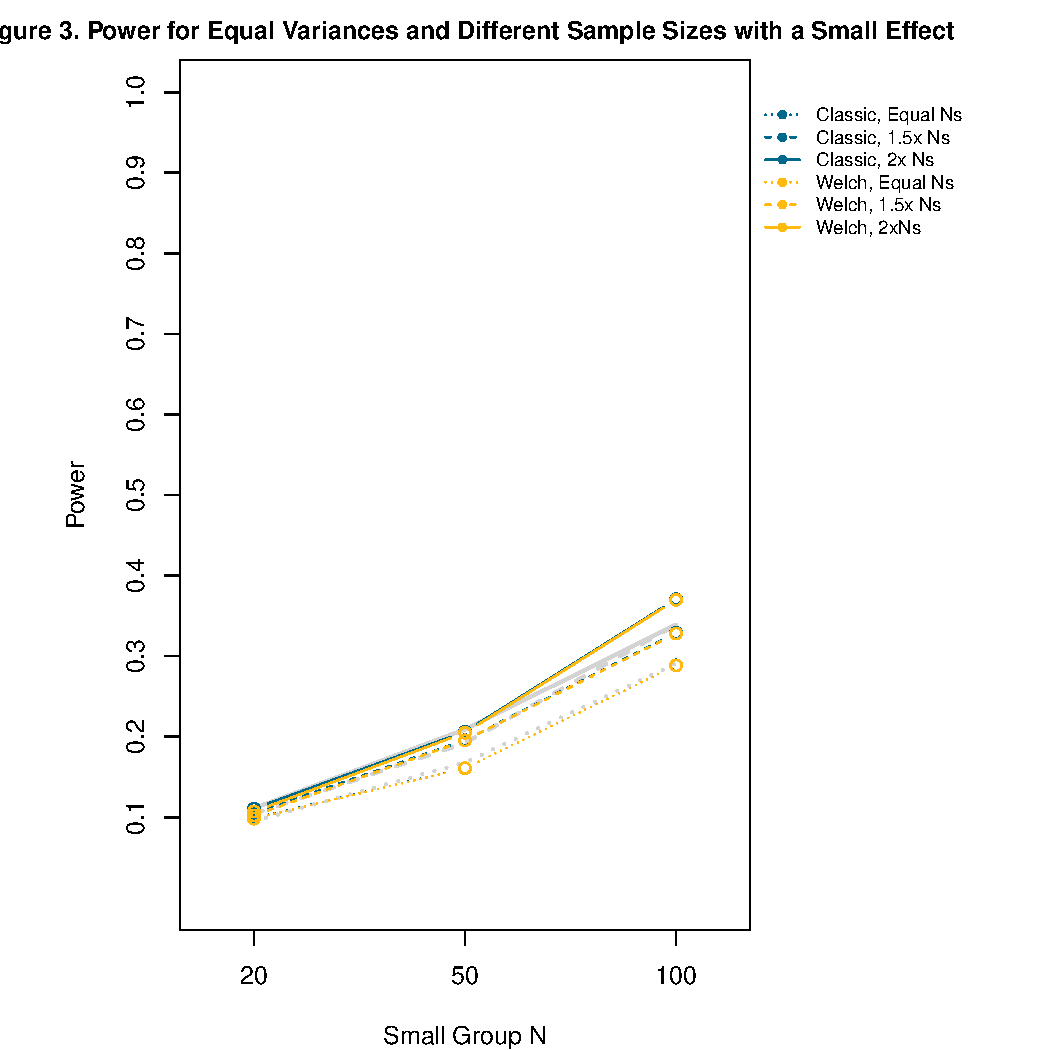
\includegraphics[width=\maxwidth]{figure/equal_vars_unequal_Ns_small_d1} 

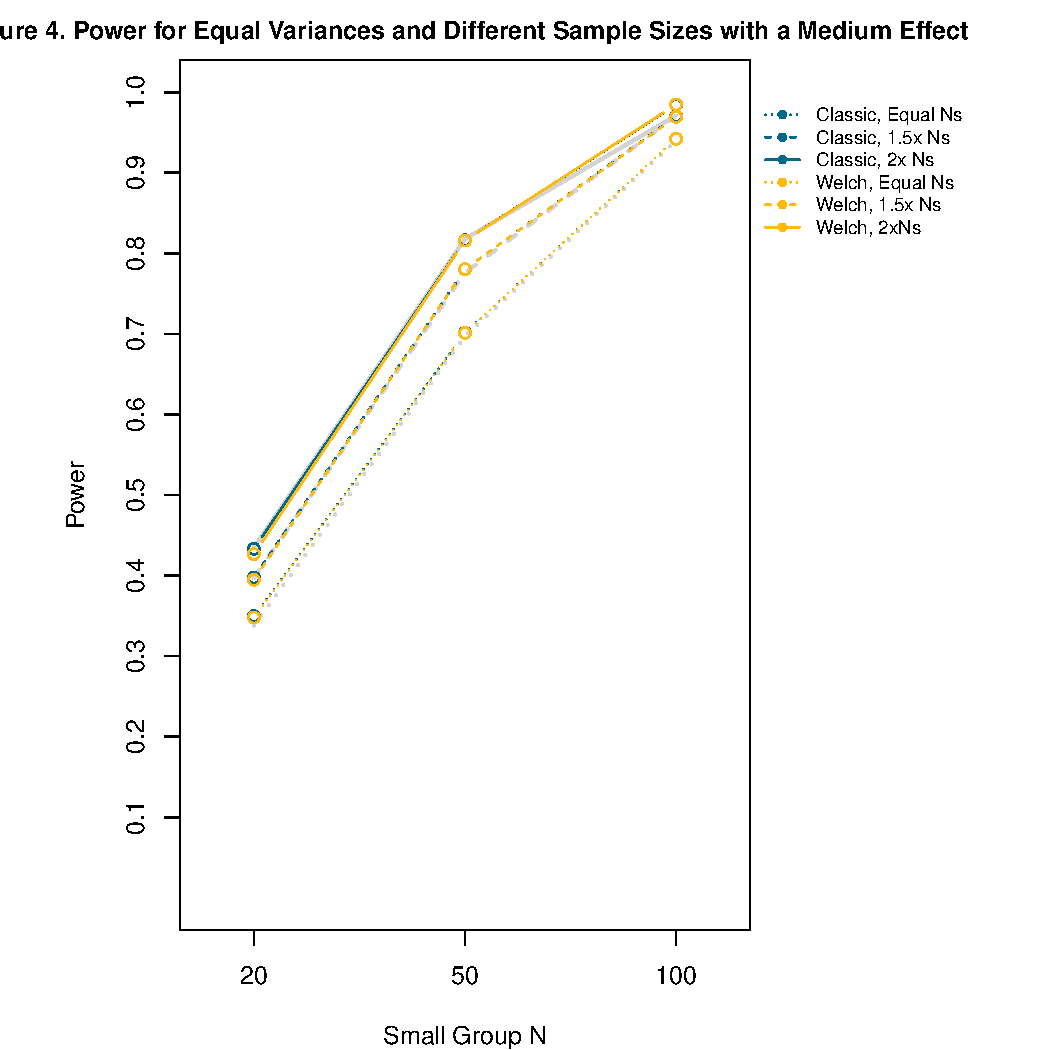
\includegraphics[width=\maxwidth]{figure/equal_vars_unequal_Ns_small_d2} 

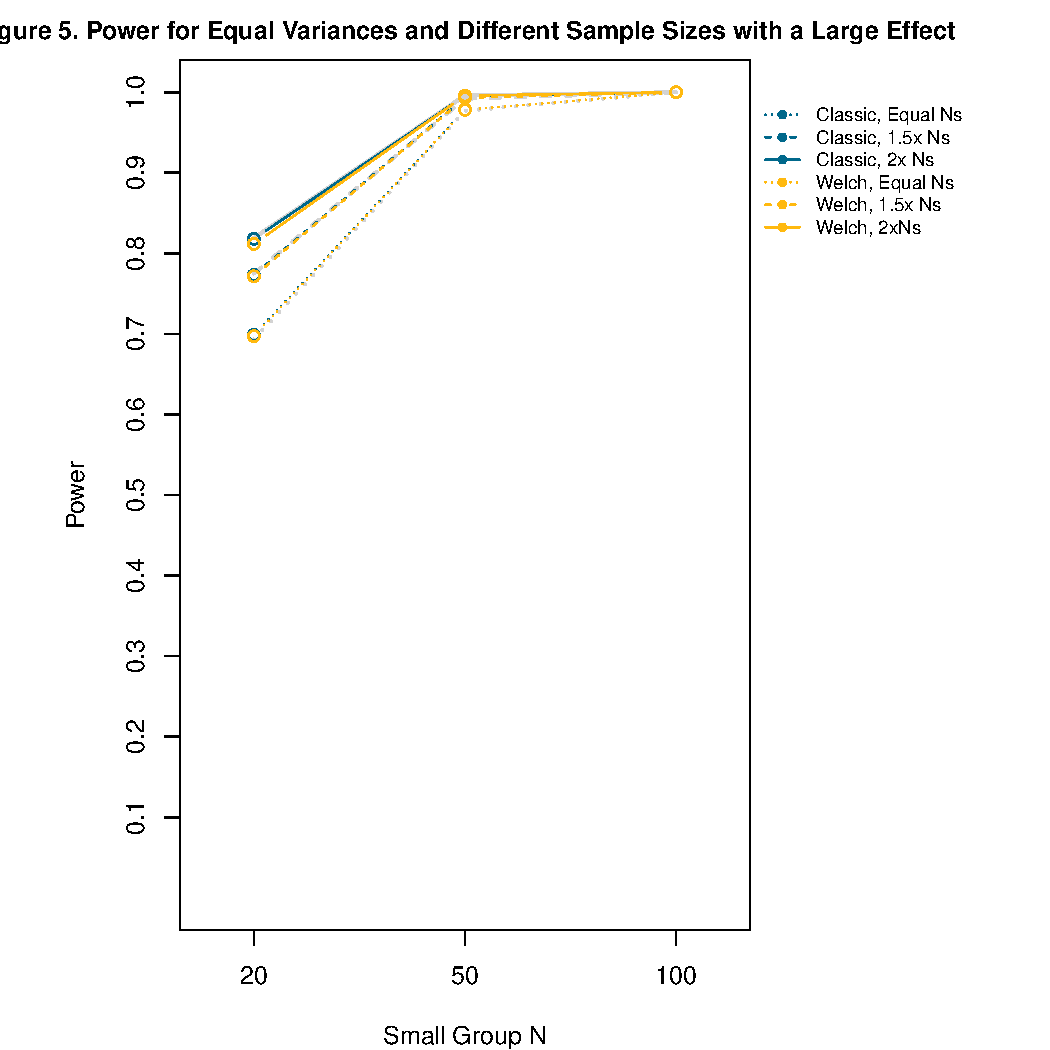
\includegraphics[width=\maxwidth]{figure/equal_vars_unequal_Ns_small_d3} 

\end{knitrout}

\subsubsection{Equal Sample Sizes, Different Variances}
Figures 6-8 display the observed power for the classic and separate variance tests when sample sizes and sample size ratios are equal, but variance ratios vary. Here too there were essentially no differences in the proportion of rejected null hypotheses (NOTE: The mean differences between groups differ by the variance ratio and power is based on a standardized effect size, not an absolute mean difference).

\begin{knitrout}
\definecolor{shadecolor}{rgb}{0.969, 0.969, 0.969}\color{fgcolor}
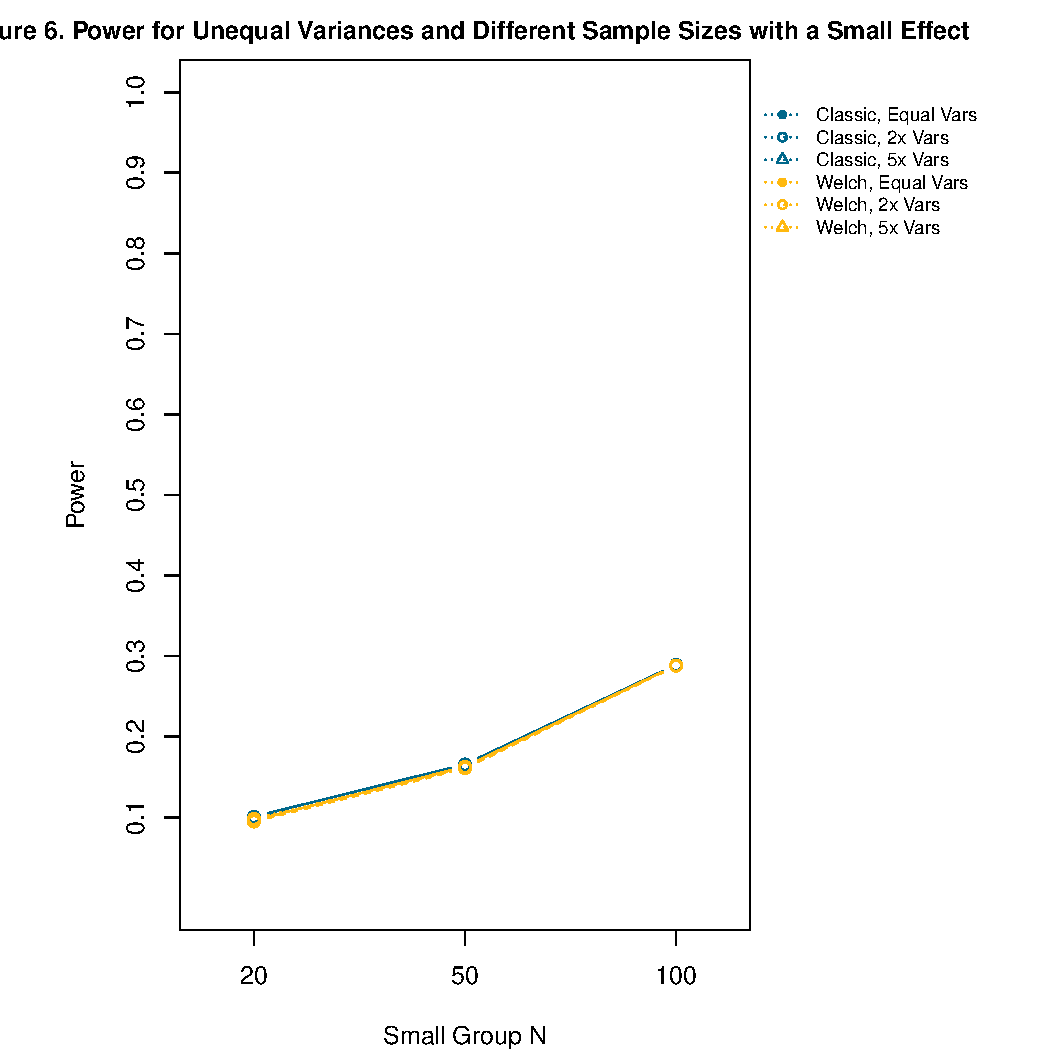
\includegraphics[width=\maxwidth]{figure/unequal_vars_equal_Ns_different_ds1} 

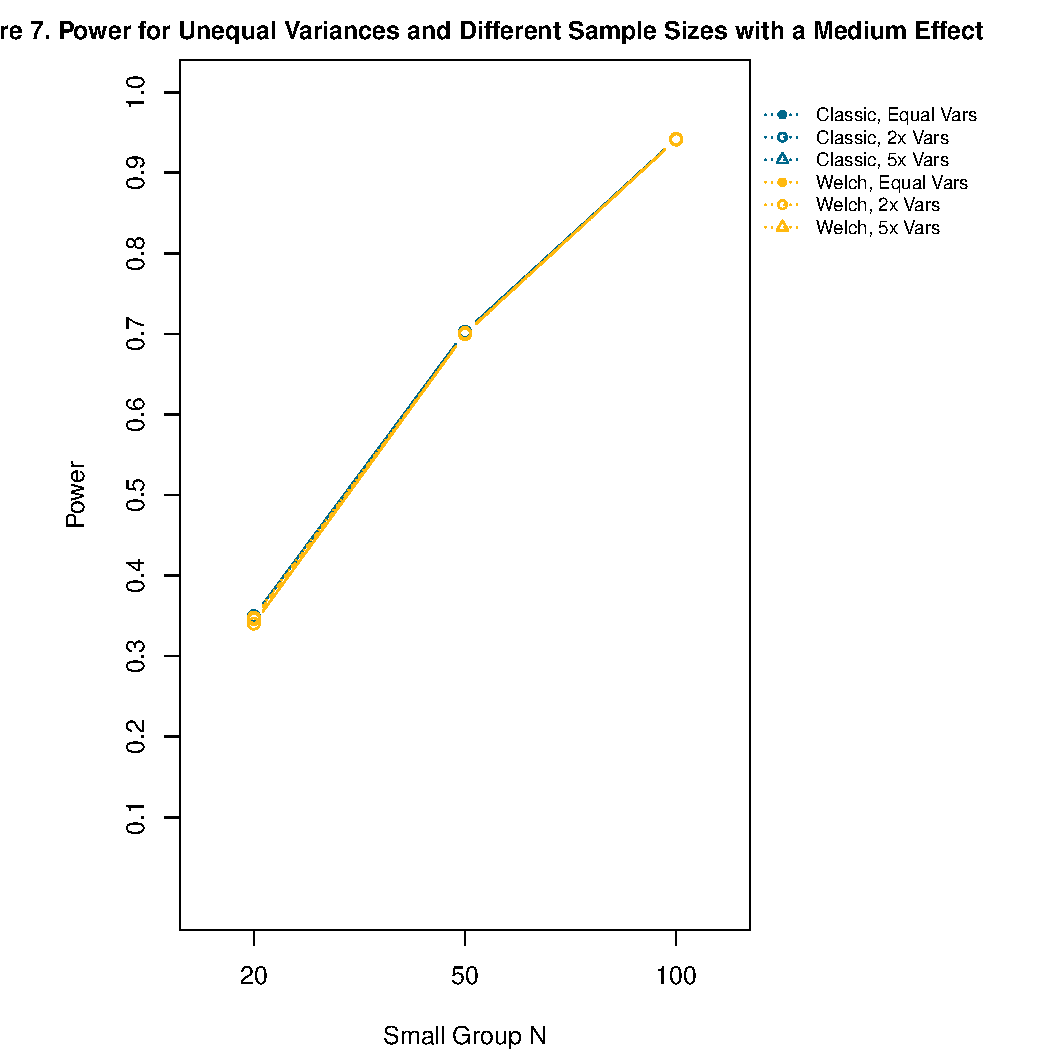
\includegraphics[width=\maxwidth]{figure/unequal_vars_equal_Ns_different_ds2} 

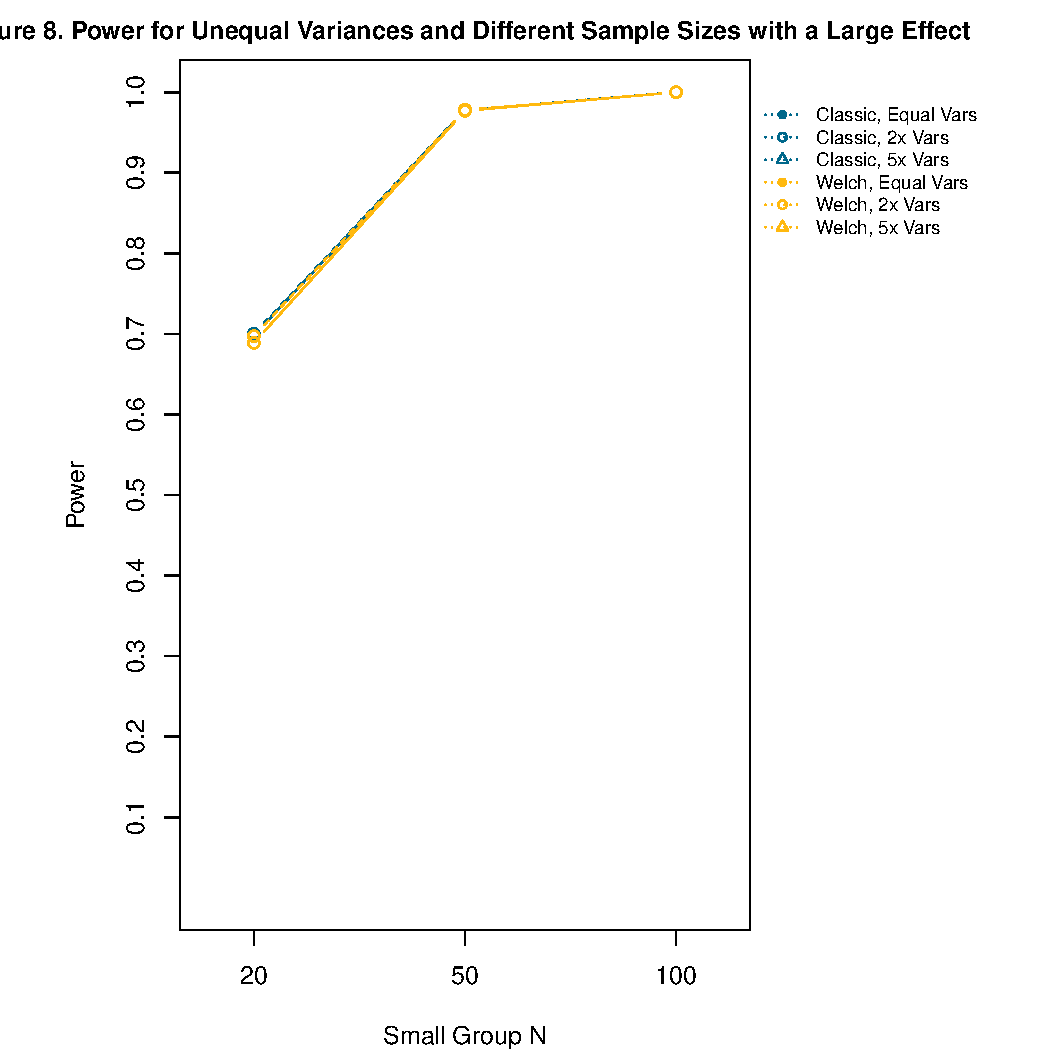
\includegraphics[width=\maxwidth]{figure/unequal_vars_equal_Ns_different_ds3} 

\end{knitrout}

\subsubsection{Different Variances, Different Ns}
The following tables display power when both variances and Ns differ.
\begin{knitrout}
\definecolor{shadecolor}{rgb}{0.969, 0.969, 0.969}\color{fgcolor}
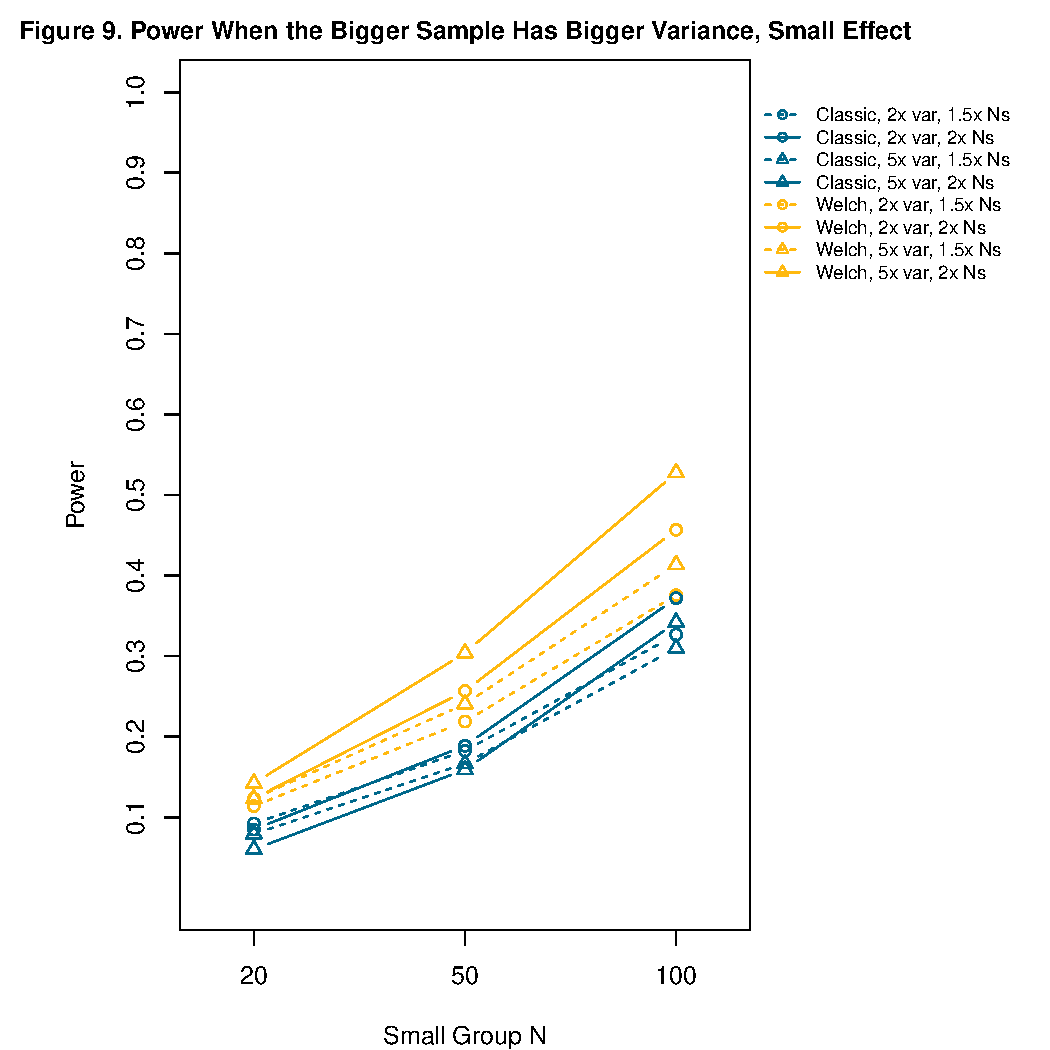
\includegraphics[width=\maxwidth]{figure/ssv_power1} 

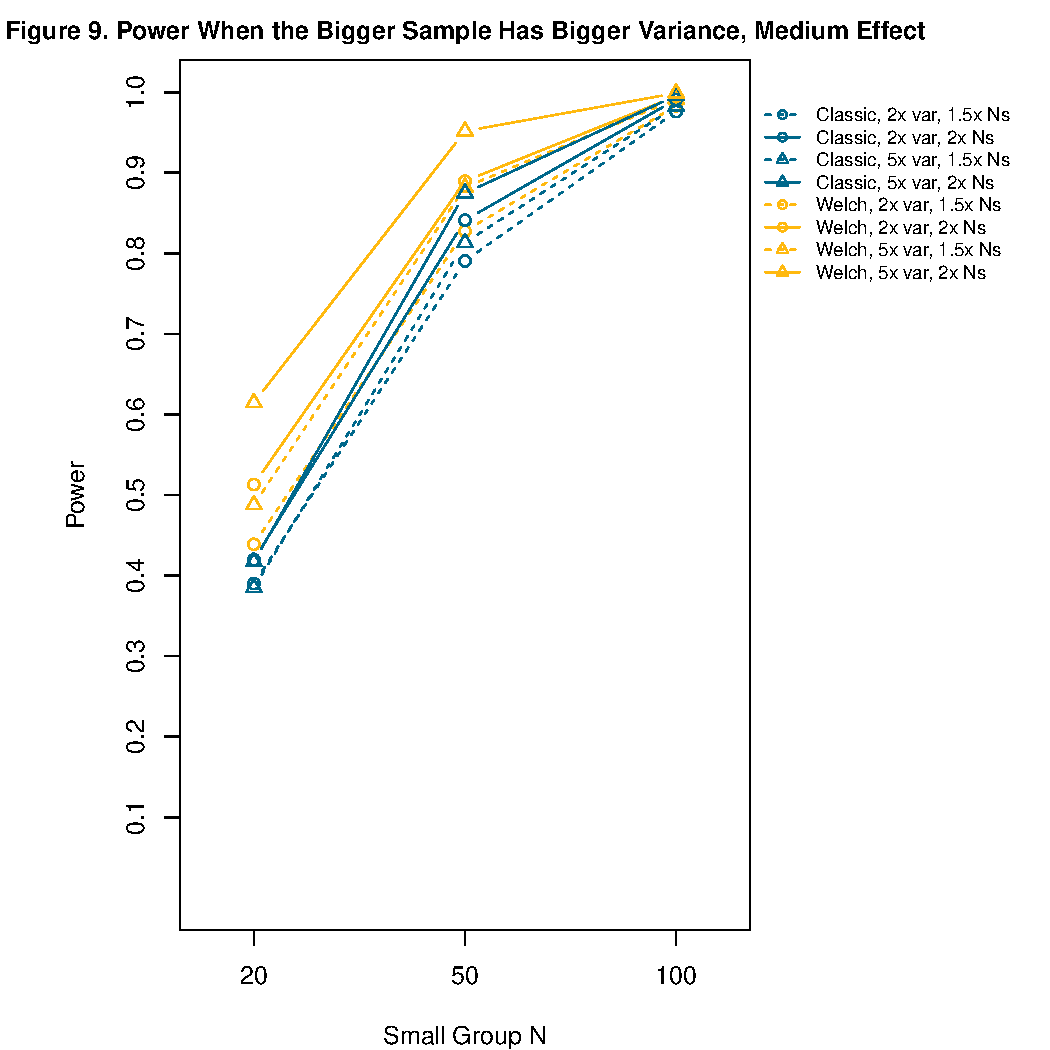
\includegraphics[width=\maxwidth]{figure/ssv_power2} 

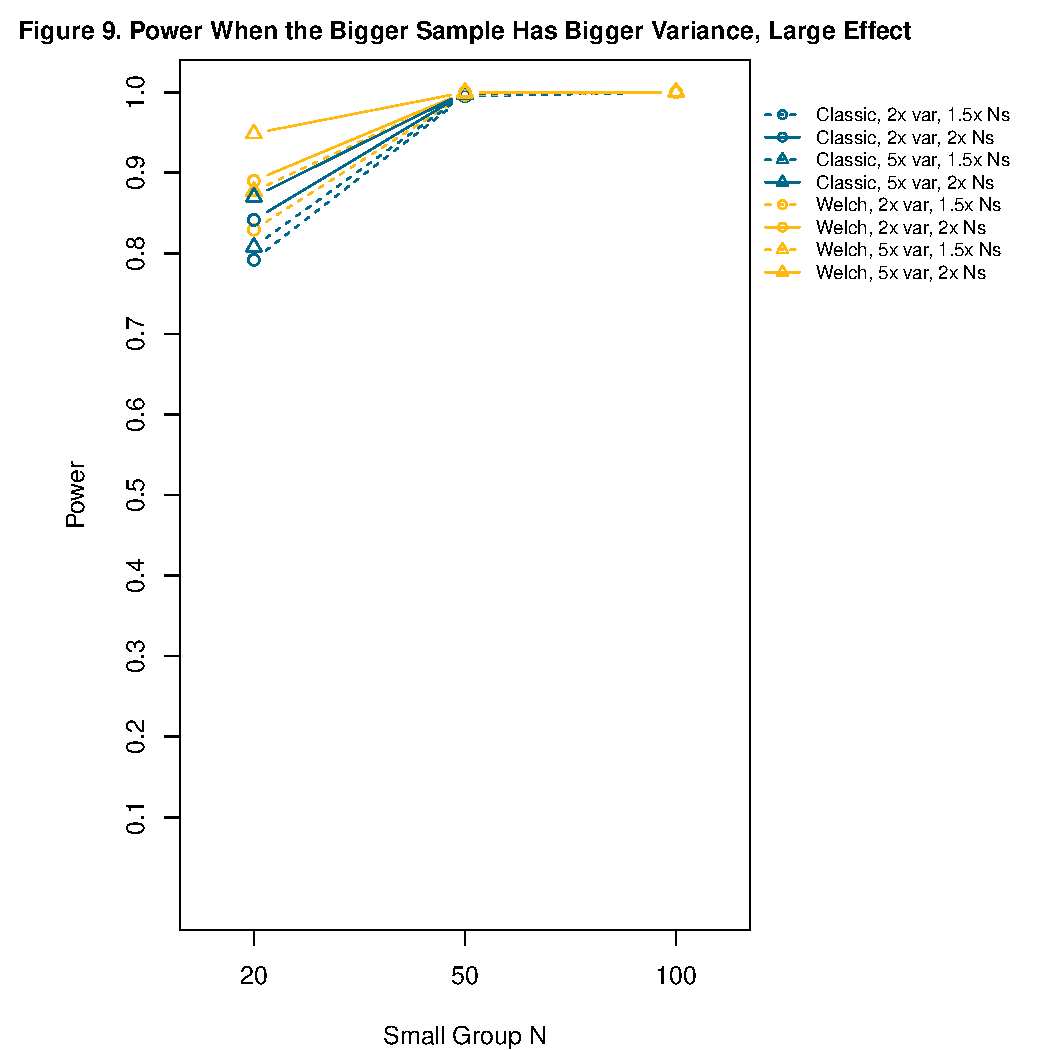
\includegraphics[width=\maxwidth]{figure/ssv_power3} 

\end{knitrout}

\subsection{Coverage Probability}


\end{document}
